\documentclass[12pt,titlepage]{extarticle}
% Document Layout and Font
\usepackage{subfiles}
\usepackage[margin=2cm, headheight=15pt]{geometry}
\usepackage{fancyhdr}
\usepackage{enumitem}	
\usepackage{wrapfig}
\usepackage{multicol}
\usepackage{caption, subcaption}

\usepackage[p,osf]{scholax}

\renewcommand*\contentsname{Table of Contents}
\renewcommand{\headrulewidth}{0pt}
\pagestyle{fancy}
\fancyhf{}
\fancyfoot[R]{$\thepage$}
\setlength{\parindent}{0cm}
\setlength{\headheight}{17pt}
\hfuzz=9pt

% Utility Management
\usepackage{color}
\usepackage{colortbl}
\usepackage{xcolor}
\usepackage{xpatch}
\usepackage{xparse}

\definecolor{links}{HTML}{1c73a5}
\definecolor{bar}{HTML}{584AA8}

% Math Packages
\usepackage{mathtools, amsmath, amsthm, thmtools, amssymb, physics}
\usepackage[scaled=1.075,ncf,vvarbb]{newtxmath}

\newcommand\B{\mathbb{B}}
\newcommand\C{\mathbb{C}}
\newcommand\R{\mathbb{R}}
\newcommand\Q{\mathbb{Q}}
\newcommand\N{\mathbb{N}}
\newcommand\Z{\mathbb{Z}}

\newcommand\Prob[1]{\mathbb{P}\qty(#1)}
\newcommand\Var[1]{\text{Var}\qty(#1)}
\newcommand\Exp[1]{\mathbb{E}\qty[#1]}
\newcommand\ball[1]{\B\qty(#1)}
\newcommand\res[1]{\underset{#1}{\operatorname{Res}}\;}
\renewcommand\pv{\mathrm{p.v.}}

\newcommand\conj[1]{\overline{#1}}
\DeclareMathOperator{\Arg}{Arg}
\DeclareMathOperator{\Log}{Log}
\DeclareMathOperator{\cis}{cis}

\DeclareMathOperator{\dom}{dom}
\DeclareMathOperator{\spann}{span}
\DeclareMathOperator{\nullity}{nullity}

\newcommand\st{\text{ s.t. }}

% TIKZ
\usepackage{tikz}
\usepackage{pgfplots}
\usetikzlibrary{arrows.meta}
\usetikzlibrary{math}
\usetikzlibrary{cd}
\usetikzlibrary{patterns}
\usetikzlibrary{decorations.markings}
\usetikzlibrary{calc}

% Boxes and Theorems
\usepackage[most]{tcolorbox}
\tcbuselibrary{skins}
\tcbuselibrary{breakable}
\tcbuselibrary{theorems}

\newtheoremstyle{default}{0pt}{0pt}{}{}{\bfseries}{\normalfont.}{0.5em}{}
\theoremstyle{default}

\renewcommand*{\proofname}{\textit{\textbf{Proof.}}}
\renewcommand*{\qedsymbol}{$\blacksquare$}
\tcolorboxenvironment{proof}{
	breakable,
	coltitle = black,
	colback = white,
	frame hidden,
	boxrule = 0pt,
	boxsep = 0pt,
	borderline west={3pt}{0pt}{bar},
	sharp corners = all,
	enhanced,
}

\newtheorem{theorem}{Theorem}[section]{\bfseries}{}
\tcolorboxenvironment{theorem}{
	breakable,
	enhanced,
	boxrule = 0pt,
	frame hidden,
	coltitle = black,
	colback = blue!7,
	left = 0.5em,
	sharp corners = all,
}

\newtheorem{corollary}{Corollary}[section]{\bfseries}{}
\tcolorboxenvironment{corollary}{
	breakable,
	enhanced,
	boxrule = 0pt,
	frame hidden,
	coltitle = black,
	colback = white!0,
	left = 0.5em,
	sharp corners = all,
}

\newtheorem{lemma}{Lemma}[section]{\bfseries}{}
\tcolorboxenvironment{lemma}{
	breakable,
	enhanced,
	boxrule = 0pt,
	frame hidden,
	coltitle = black,
	colback = green!7,
	left = 0.5em,
	sharp corners = all,
}

\newtheorem{definition}{Definition}[section]{\bfseries}{}
\tcolorboxenvironment{definition}{
	breakable,
	coltitle = black,
	colback = white,
	frame hidden,
	boxsep = 0pt,
	boxrule = 0pt,
	borderline west = {3pt}{0pt}{orange},
	sharp corners = all,
	enhanced,
}

\newtheorem{example}{Example}[section]{\bfseries}{}
\tcolorboxenvironment{example}{
	% title = \textbf{Example},
	% detach title,
	% before upper = {\tcbtitle\quad},
	breakable,
	coltitle = black,
	colback = white,
	frame hidden,
	boxrule = 0pt,
	boxsep = 0pt,
	borderline west={3pt}{0pt}{green!70!black},
	sharp corners = all,
	enhanced,
}

\newtheoremstyle{remark}{0pt}{4pt}{}{}{\bfseries\itshape}{\normalfont.}{0.5em}{}
\theoremstyle{remark}
\newtheorem*{remark}{Remark}


% TColorBoxes
\newtcolorbox{week}{
	colback = black,
	coltext = white,
	fontupper = {\large\bfseries},
	width = 1.2\paperwidth,
	size = fbox,
	halign upper = center,
	center
}

\newcommand{\banner}[2]{
    \pagebreak
    \begin{week}
   		\section*{#1}
    \end{week}
    \addcontentsline{toc}{section}{#1}
    \addtocounter{section}{1}
    \setcounter{subsection}{0}
}

% Hyperref
\usepackage{hyperref}
\hypersetup{
	colorlinks=true,
	linktoc=all,
	linkcolor=links,
	bookmarksopen=true
}


\def\homeworknumber{4}
\usepackage{fancyhdr}
\pagestyle{fancy}
\fancyhead[R]{HW \#\thehwnumber}
\fancyhead[C]{\textbf{Math 130B}}
\fancyhead[L]{Eli Griffiths}


\begin{document}

% Section 46: 1, 8, 10, 13
% Section 47: 3, 6
% Section 49: 2, 5
% Section 53: 2, 3, 7
% Section 57: 1, 3, 6, 10
% Section 59: 1

\subsection*{46.1}
\subsubsection*{Part A}
\begin{align*}
    \int_C f(z) \dd z &= \int_0^\pi \qty(1 + \frac{2}{2 e^{i \theta}}) \dv{\theta}(2e^{i \theta}) \dd \theta \\
    &= \int_0^\pi \qty(1 + e^{-i \theta})\qty(2i e^{i \theta}) \dd \theta \\
    &= \int_0^\pi \qty(2i e^{i \theta} + 2i) \dd \theta \\
    &= \qty[2e^{i \theta} + 2i \theta]_0^\pi \\
    &= 2e^{i \pi} + 2 \pi i - 2e^{0} + 0 \\
    &= -4 + 2 \pi i
\end{align*}

\subsubsection*{Part B}
\begin{align*}
    \int_C f(z) \dd z &= \int_\pi^{2 \pi} \qty(1 + \frac{2}{2 e^{i \theta}}) \dv{\theta}(2e^{i \theta}) \dd \theta \\
    &= \int_\pi^{2 \pi} \qty(1 + e^{-i \theta})\qty(2i e^{i \theta}) \dd \theta \\
    &= \int_\pi^{2 \pi} \qty(2i e^{i \theta} + 2i) \dd \theta \\
    &= \qty[2e^{i \theta} + 2i \theta]_{\pi}^{2 \pi} \\
    &= 2e^{2 \pi i} + 4 \pi i - 2e^{\pi i} - 2 \pi i \\
    &= 2 + 4 \pi i + 2 - 2 \pi i \\
    &= 4 + 2 \pi i
\end{align*}

\subsubsection*{Part C}
\begin{align*}
    \int_C f(z) \dd z &= \int_0^{2 \pi} \qty(1 + \frac{2}{2 e^{i \theta}}) \dv{\theta}(2e^{i \theta}) \dd \theta \\
    &= \int_0^{2 \pi} \qty(1 + e^{-i \theta})\qty(2i e^{i \theta}) \dd \theta \\
    &= \int_0^{2 \pi} \qty(2i e^{i \theta} + 2i) \dd \theta \\
    &= \qty[2e^{i \theta} + 2i \theta]_{0}^{2 \pi} \\
    &= 2e^{2 \pi i} + 4 \pi i - 2 e^{0} - 0 \\
    &= 2 + 4 \pi i - 2 \\
    &= 4 \pi i
\end{align*}

\subsection*{46.8}
$C$ can be parameterized by the function
\[
    z(\theta) = R e^{i \theta}, - \pi \leq \theta \leq \pi
\]
meaning
\[
    f(z(\theta)) = \exp[(a-1) \Log(R e^{i \theta})] = \exp[(a-1)(\ln R + i \theta)]
.\]
Therefore
\begin{align*}
    \int_C f(z) \dd z &= \int_{-\pi}^{\pi} \exp[(a-1)(\ln R + i \theta)] \qty(iR e^{i \theta}) \dd \theta \\
                      &= i R e^{(a-1) \ln R} \int_{-\pi}^\pi e^{i a \theta} \dd \theta \\
                      &= i R R^{a-1} \cdot \frac{1}{i a} \qty[e^{i a \theta}]_{-\pi}^{\pi} \\
                      &= \frac{R^a}{a} (e^{a \pi i} - e^{-a \pi i}) \\
                      &= i\frac{2R^a}{a} \sin(a \pi)
\end{align*}


\subsection*{46.10}
Parameterize the contour $C$ with $z(\theta) = e^{i \theta}$ with $0 \leq \theta \leq 2 \pi$. Then
\begin{align*}
    \int_C z^m \conj{z}^n \dd z = \int_0^{2 \pi} \qty(e^{im \theta} e^{-in \theta})\qty(ie^{i \theta}) \dd \theta &= i \int_0^{2 \pi} e^{i(m + 1)\theta} e^{-in \theta} \dd \theta \\
    &= i \begin{cases}
        0 & m + 1 \neq n \\
        2 \pi & m + 1 = n
    \end{cases} \\
    &= \begin{cases}
        0 & m + 1 \neq n \\
        2 \pi i & m + 1 = n
    \end{cases}
\end{align*}

\subsection*{46.13}
\begin{proof}
    Let $f(z) = (z - z_0)^{n-1}$ and $z(t) = z_0 + Re^{i t}$. Note then that
    \[
        f(z(t)) = \qty(z_0 + Re^{i t} - z_0)^{n-1} = R^{n-1} e^{it(n-1)}
    \]
    and
    \[
        z'(t) = Ri e^{it}
    .\]
    Therefore
    \begin{align*}
        \int_{C_0} (z-z_0)^{n-1} \dd z &= \int_{-\pi}^{\pi} \qty(R^{n-1} e^{it(n-1)})\qty(R i e^{it}) \dd t \\
                                       &= i R^n \int_{-\pi}^{\pi} e^{itn} \dd t
    \end{align*}
    Consider two cases
    \begin{enumerate}[leftmargin=2cm]
        \item[$(n = 0)$]
            The integral equals
            \[
                iR^0 \int_{-\pi}^{\pi} e^{it (0)} \dd t = i \int_{\pi}^{\pi} \dd t = 2 \pi i
            .\]
        \item[$(n \neq 0)$]
            The integral equals
                \[
                    iR^n \int_{-\pi}^{\pi} e^{itn} = iR^n \qty[\frac{e^{itn}}{i n}]_{-\pi}^\pi = \frac{R^n}{n} \qty[e^{in(\pi)} - e^{in(-\pi)}] = \frac{R^n}{n} \qty[-1 - (-1)] = 0
                .\]
    \end{enumerate}
    Therefore
    \[
        \int_{C_0} (z-z_0)^{n-1} \dd z = \begin{cases}
            0 & n \in \Z \setminus \qty{0} \\
            2 \pi i & n = 0
        \end{cases} \qedhere
    \]
\end{proof}

\subsection*{47.3}
\begin{wrapfigure}{r}{6cm}
\begin{tikzpicture}
    \draw (-4.5, 0) -- (0.5, 0) node[anchor=west] {$\Re z$};
    \draw (0, -0.5) -- (0, 3.5) node[anchor=south] {$\Im z$};
    \draw[thick, dashed] (0, 0) rectangle (-4, 3) node[anchor=south east] {$-4 + 3i$};
    \fill[black] (-4, 3) circle[radius = 2pt];
    \begin{scope}[very thick,decoration={
        markings,
        mark=at position 0.5 with {\arrow{>}}}
        ] 
        \draw[postaction={decorate}] (0,0) -- (0, 3);
        \draw[postaction={decorate}] (0, 3) -- (-4, 0);
        \draw[postaction={decorate}] (-4, 0) -- (0, 0);
    \end{scope}
    \draw (-1.2, 1) node {$C$};
\end{tikzpicture}
\end{wrapfigure}

The entire contour can be bounded by the rectangle from $0$ to $-4 + 3i$. Therefore for $z = x + iy$ it follows on $C$ that $-4 \leq x \leq 0$ and $0 \leq y \leq 3$. Since $|e^z - \conj{z}| \leq e^{x} + \sqrt{x^2 + y^2}$
\[
    |e^z - \conj{z}| \leq e^x + \sqrt{x^2 + y^2} \leq e^0 + \sqrt{(-4)^2 + 3^2} = 6
\]
when $z$ is in the rectangle. Since the length of the path is $4 + 3 + \sqrt{3^2 + (-4)^2} = 3 + 4 + 5 = 12$, it follows that
\[
    \qty|\int_C e^z - \conj{z}| \leq 5 \cdot 12 = 60
.\]

\subsection*{47.6}
\begin{proof}
    When on $C_{\rho}$, $|z^{\frac{1}{2}}| = \sqrt{\rho}$ and therefore $\qty|z^{-\frac{1}{2}}| = \frac{\sqrt{\rho}}{\rho}$. Since $f(z)$ is analytic on the disk $|z| \leq 1$, then there exists some $M \in \R > 0$ such that $|f(z)| \leq M$ for all $z$ on the disk. Therefore
    \[
        \qty|z^{-\frac{1}{2}} f(z)| \leq \frac{M \sqrt{\rho}}{\rho}
    .\]
    $z^{-\frac{1}{2}}$ is analytic on any branch taken and so $z^{-\frac{1}{2}} f(z)$ is analytic and hence piecewise continuous on $C_{\rho}$. Therefore
    \[
        \int_{C_{\rho}} \qty(z^{-\frac{1}{2}} f(z)) \leq 2 \pi \rho \cdot \frac{M \sqrt{\rho}}{\rho} = 2 \pi M \sqrt{\rho}
    .\]
    Therefore since $\lim_{\rho \to 0} 2 \pi M \sqrt{ \rho } = 0$, then
    \[
        \lim_{\rho \to 0} \qty|\int_{C_{\rho}} z^{-\frac{1}{2}} f(z)| = 0 \implies \lim_{\rho \to 0} \int_{C_{\rho}} z^{-\frac{1}{2}} f(z) = 0
    .\]
\end{proof}

\subsection*{49.2}
\subsubsection*{Part A}
Note that $F(z) = \frac{z^3}{3}$ is an antiderivative of $z^2$ since $\dv{z} \frac{z^{3}}{3} = 3 \cdot \frac{x^2}{3} = x^2$. Therefore the integral is 
\[
    \int_0^{1+i} z^2 \dd z = \qty[\frac{z^3}{3}]_0^{1+i} = \frac{(1+i)^3}{3} = \frac{-2 - 2 i}{3} = \frac{2}{3} (-1 - i)
.\]

\subsubsection*{Part B}
Note that $F(z) = 2\sin(\frac{z}{2})$ is an antiderivative of $\cos(\frac{z}{2})$ since $\dv{z} 2 \sin(\frac{z}{2}) = 2 \cdot \frac{1}{2} \cdot \cos(\frac{z}{2}) = \cos(\frac{z}{2})$. Therefore the integral is 
\begin{align*}
    \int_0^{\pi + 2i} \cos(\frac{z}{2}) \dd z &= 2\qty[\sin(\frac{z}{2})]_0^{\pi + 2i} \\
    &= 2 \sin(\frac{\pi}{2} + i) \\
    &= 2 \qty(\frac{e^{i\qty(\frac{\pi}{2} + i)} - e^{-i\qty(\frac{\pi}{2} + i)}}{2i}) \\
    &= \frac{e^{-1}e^{i \frac{\pi}{2}} - e^{1} e^{-i \frac{\pi}{2}}}{i} \\
    &= \frac{e^{-1}i + e^{1}i}{i} \\
    &= \frac{1}{e} + e
\end{align*}

\subsubsection*{Part C}
Note that $F(z) = \frac{1}{4}(z-2)^4$ is an antiderivative of $(z-2)^3$ since $\dv{z}(\frac{1}{4}(z-2)^4) = 4 \cdot \frac{1}{4} (z-2)^3 = (z-2)^3$. Therefore the integral is
\[
    \int_1^3 (z-2)^3 \dd z = \frac{1}{4} \qty[(z-2)^4]_1^3 = \frac{1}{4} \qty[1 - 1] = 0
.\]

\subsection*{49.5}
Let $\gamma$ be a path from $-1$ to $1$ above the real axis. Note then that for any $z \in \gamma$ that $0 \leq \Arg z \leq \pi$. Therefore for all $z \in \gamma$ except $z = -1$, the branches $(-\pi, \pi)$ and $(-\frac{\pi}{2}, \frac{3 \pi}{2})$ agree value wise. Using this branch of $\log$ gives an anti derivative valid on all of $\gamma$ that agrees with the principal branch
\[
    F(z) = \frac{1}{i} \exp[i \log z] = \frac{1}{i+1} z^{i+1}
.\]
Therefore
\begin{align*}
    \int_{-1}^{1} z^i \dd z &= F(1) - F(-1)  \\
    &= \frac{1}{i+1} \qty(\exp[(1+i) \log 1] - \exp[(1+i) \log(-1)])  \\
    &= \frac{1}{i+1} \qty(\exp[0] - \exp[(1+i)(\ln 1 + i\pi)])  \\
    &= \frac{1}{i+1} \qty(1 - e^{\ln 1} e^{i \pi} e^{-\pi} e^{i \ln 1}) \\
    &= \frac{1}{i+1} \qty(1 - 1(-1) e^{-\pi}(1)) \\
    &= \frac{1}{i+1} \qty(1 + e^{-\pi}) \\
    &= \frac{i - 1}{(i+1)(i-1)} \qty(1 + e^{-\pi}) \\
    &= \frac{i - 1}{2} \qty(1 + e^{-\pi}) \\
    &= \frac{1 + e^{-\pi}}{2} (i - 1)
\end{align*}

\subsection*{53.2}
\subsubsection*{Part A}
Since $f(z)$ is a composition of an entire function and a $\frac{1}{z}$, $f(z)$ will be analytic everywhere except when $3z^2 + 1 = 0 \implies z^2 = -\frac{1}{3} \implies z = \pm \frac{i}{\sqrt{3}}$. Since these points are not in closed region between $C_1$ and $C_2$, then curve deformation can be applied to get $\int_{C_1} f(z) \dd z = \int_{C_2} f(z) \dd z$.

\subsubsection*{Part B}
The only place where $f(z)$ is not analytic is when $\sin(\frac{z}{2}) = 0$ which is when $z = 2 \pi k$ for $k \in \Z$. The closest zeroes are then $0, 2 \pi$ and $-2 \pi$ which are all not inside the region between $C_1$ and $C_2$. Therefore $f$ is analytic in the region between the contours and hence the integral paths can be deformed into each other.


\subsubsection*{Part C}
The only place where $f(z)$ is not analytic is when $1 - e^{z} = 0$ which is at $z=0$. Since $z = 0$ is not in the region between $C_1$ and $C_2$, $f$ is analytic in the region and therefore the integral paths can be deformed into each other.

\subsection*{53.3}
Consider a circular contour $C_0$ of radius $R = 10$ centered around $2 + i$. Note that the given rectangular contour is contained inside the circle. Since $(z-2-i)^{n-1}$ is entire, the region between these contours is entire and therefore the integral around the rectangular path equals the integral around the circular path. Therefore
\[
    \int_C (z - 2 - i)^{n-1} \dd z = \int_{C_0} (z-z_0)^{n-1} \dd z = \begin{cases}
        0 & n \in \Z \\
        2 \pi i & n = 0
    \end{cases}
.\]

\subsection*{53.7}
\begin{proof}
    Since $\conj{z} = x - iy$ for $z = x + iy$, then its partials are
    \begin{alignat*}{3}
        u_x &= 1 \hspace{1cm}&& v_x &&= 0 \\
        u_y &= 0 && v_y &&= -1
    \end{alignat*}
    Let $\mathcal{R}$ denote the region enclosed by the contour $C$. Then
    \begin{align*}
        \frac{1}{2i} \int_C \conj{z} \dd z &= \frac{1}{2i} \qty[\iint_{\mathcal{R}} (-v_x - u_y) \dd A + i \iint_{\mathcal{R}} (u_x - u_y) \dd A] \\
        &= \frac{1}{2i} \qty[
            \iint_{\mathcal{R}} 0 \dd A + i \iint_{\mathcal{R}} 2 \dd A
        ] \\
        &= \frac{2}{2i} \cdot i \iint_{\mathcal{R}} \dd A \\
        &= \iint_{\mathcal{R}} \dd A = \text{area of } \mathcal{R} \qedhere
    \end{align*}
\end{proof}

\subsection*{57.1}
Rewriting Cauchy Integral Formula and it's extension gives
\[
    \int_C \frac{f(z)}{z - z_0} \dd z = 2 \pi i f(z_0)
\]
and
\[
    \int_C \frac{f(z)}{(z - z_0)^{n+1}} \dd z = \frac{2 \pi i}{n!} f^{(n)}(z_0)
.\]

\subsubsection*{Part A}
Let $f(z) = e^{-z}$ and $z_0 = \frac{\pi i}{2}$. Note $f(z)$ is entire and therefore analytic on and in the contour $C$. Then
\[
    \int_C \frac{e^{-z}}{z - \frac{\pi i}{2}} \dd z = \int_C \frac{f(z)}{z - z_0} \dd z = 2 \pi i f(z_0) = 2 \pi i e^{-\frac{\pi i}{2}} = 2 \pi i (-i) = 2 \pi
.\]

\subsubsection*{Part B}
Let $f(z) = \frac{\cos z}{z^2 + 8}$ and $z_0 = 0$. Since $\cos z$ is entire, $f(z)$ is not analytic only when $z^2 + 8 = 0$ which occurs at $z = \pm \sqrt{8}$ which is outside of the contour. Therefore $f(z)$ is analytic on and in the contour. Then
\[
    \int_C \frac{\cos z}{z(z^2 + 8)} \dd z = \int_C \frac{f(z)}{z - z_0} \dd z = 2 \pi i f(z_0) = 2 \pi i \cdot \frac{\cos 0}{0^2 + 8} = \frac{2 \pi i}{8} = \frac{\pi i}{4}
.\]

\subsubsection*{Part C}
Let $f(z) = \frac{z}{2}$ and $z_0 = -\frac{1}{2}$. Since $f(z)$ is entire, $f(z)$ is analytic on and in the contour. Then
\[
    \int_C \frac{z}{2z + 1} \dd z = \int_C \frac{\frac{z}{2}}{z + \frac{1}{2}} \dd z = \int_C \frac{\frac{z}{2}}{z - \qty(-\frac{1}{2})} \dd z = \int_C \frac{f(z)}{z - z_0} \dd z = 2 \pi i f(z_0) = -2 \pi i \cdot \frac{1}{4} = - \frac{\pi i }{2}
.\]

\subsubsection*{Part D}
Let $f(z) = \cosh(z)$ and $z_0 = 0$. Since $f(z)$ is entire, then it's derivatives are entire and hence analytic on and in the contour. Note that $f^{(3)}(z) = \dv[3]{z} \cosh z = \sinh z$. Then
\[
    \int_C \frac{\cosh z}{z^4} \dd z = \int_C \frac{\cosh z}{(z-0)^{3 + 1}} \dd z = \int_C \frac{f(z)}{(z - z_0)^{3 + 1}} \dd z = \frac{2 \pi i}{3!} f^{(3)}(z_0) = \frac{\pi i}{3} \cdot \sinh 0 = 0
.\]

\subsubsection*{Part E}
Let $f(z) = \tan(\frac{z}{2})$ and $z_0 = x_0$. Since $f(z)$ is analytic for $-\pi < \Re z < \pi$ and $-\pi < -2 \leq \Re z \leq 2 < \pi$ in and on $C$, it follows that $f(z)$ is analytic on and in $C$. Then
\[
    \int_C \frac{\tan(\frac{x}{2})}{(z-x_0)^2} \dd z = \int_C \frac{f(z)}{(z-z_0)^{1+1}} \dd z = \frac{2 \pi i}{1!} f'(z_0) = 2 \pi i \cdot \frac{1}{2} \sec[2](\frac{z_0}{2}) = \pi i \sec[2](\frac{x_0}{2})
.\]

\subsection*{57.3}
\begin{align*}
    g(2) &= \int_C \frac{2s^2 - s - 2}{s - 2} \dd s \\
    \intertext{Since $2s^2 - s - 2$ is entire, then it is analytic on and inside of $C$ meaning}
    &= 2 \pi i \qty(2 \cdot 2^2 - 2 - 2) \\
    &= 2 \pi i \cdot 2^2 \\
    &= 8 \pi i
\end{align*}

If $|z| > 3$, then $\frac{2s^2 - s - 2}{s - z}$ will be analytic in an on the curve since the boundary and interior of the curve is when $|z| < 3$. Therefore since the integrand is analytic and the integral is over a closed contour, then the integral will be $0$ meaning $g(z) = 0$ for $|z| > 3$.


\subsection*{57.6}
\begin{proof}
    Let $z$ be a point on the interior of $C$ and $d = \inf\qty{|z - s| : s \in C}$. Choose $\Delta z$ such that $0 < |\Delta z| < d$ since $d \neq 0$. It follows then that
    \[
        \frac{g(z + \Delta z) - g(z)}{\Delta z} = \frac{1}{2 \pi i} \int_C \qty(\frac{1}{s - z - \Delta z} - \frac{1}{s - z}) \frac{f(s)}{\Delta z} \dd s
    .\]
    Since $\frac{1}{s - z - \Delta z} - \frac{1}{s - z} = \frac{\Delta z}{(s - z - \Delta z)(s -z)}$, it follows
    \[
        \frac{g(z + \Delta z) - g(z)}{\Delta z} = \frac{1}{2 \pi i} \int_C \frac{f(s)}{(s - z - \Delta z)(s -z)} \dd s
    .\]
    Rewriting $\frac{1}{(s - z - \Delta z)(s - z)} = \frac{1}{(s-z)^2} + \frac{\Delta z}{(s - z - \Delta z)(s-z)^2}$ gives
    \[
        \frac{g(z + \Delta z) - g(z)}{\Delta z} - \frac{1}{2 \pi i} \int_C \frac{f(s)}{(s-z)^2} \dd s = \frac{1}{2 \pi i} \int_C \frac{\Delta z f(s)}{(s - z - \Delta z)(s - z)^2} \dd s
    . \tag{$\star$}\]
    Since $f(z)$ is continuous on the simple closed contour $C$ and a simple closed contour is a compact set, it follows that $|f(z)|$ is bounded by some $M$. Since $|s - z| \geq d$ and $|\Delta z| < d$ for $s \in C$, the inequality
    \[
        |s - z - \Delta z| = |(s-z) - \Delta z| \geq ||s-z| - |\Delta z|| \geq d - |\Delta z| > 0
    \]
    holds. Therefore
    \[
        \qty|\frac{1}{2 \pi i} \int_C \frac{\Delta z f(s)}{(s - z - \Delta z)(s - z)^2} \dd s| \leq \frac{|\Delta z| M L}{(d - |\Delta z|)d^2}
    \]
    where $L$ denotes the length of $C$. Since
    \[
        \lim_{\Delta z \to 0} \frac{|\Delta z| M L}{(d - |\Delta z|)d^2} = 0
    \]
    it follows that the left hand side of $(\star)$ has the same limit meaning
    \[
        g'(z) = \lim_{\Delta z \to 0} \frac{g(z + \Delta z) - g(z)}{\Delta z} = \frac{1}{2 \pi i} \int_C \frac{f(s)}{(s - z)^2} \dd s
    .\]
    Therefore since $z$ was an arbitrary interior point to $C$, $g'(z)$ exists on the interior of $C$. Furthermore, since every $z \in C$ has an open ball around it in $C$, then every $z$ has a neighborhood that is differentiable meaning $g(z)$ is analytic on the interior of $C$.
\end{proof}


\subsection*{57.10}
\begin{proof}
    Consider a positively oriented circular contour $C_R$ around some $z_0 \in \C$ with radius $R$. Note that for all $z \in C_R$ that $|z| \leq |z_0| + R$. Therefore $A|z| \leq A(|z_0| + R)$ on the contour, giving an upper bound of $f$ on $C_R$. Since $f$ is entire, then it is analytic in and on $C_R$ meaning
    \[
        |f''(z_0)| \leq \frac{2! \cdot A (|z_0| + R)}{R^n} = 2\qty(\frac{A |z_0|}{R^n} + \frac{1}{R^{n-1}})
    .\]
    Since $R$ was chosen arbitrarily and $\lim_{R \to \infty} 2\qty(\frac{A |z_0|}{R^n} + \frac{1}{R^{n-1}}) = 2 (0 + 0) = 0$, it follows that $|f''(z_0)| = 0 \implies f''(z_0) = 0$ for all $z_0 \in \C$. Therefore $f(z) = a_1x + b_1$ for some $a_1, b_1 \in \C$. Since $|f(0)| \leq A \cdot 0$, it follows that $b_1 = 0$. Therefore $f(z) = a_1 x$ for all $z$.
\end{proof}

\subsection*{59.1}
\begin{proof}
    Take $f(z)$ to be entire and assume that there is an upper bound $u_0$ for $u(x,y) = \Re f$ on all of $\C$. Consider the function $g(z) = e^{f(z)}$. Since $e^z$ and $f(z)$ are entire, then $g(z)$ is also entire. Note that
    \[
        g(z) = \exp[f(z)] = \exp[u(x,y) + iv(x,y)] = \exp[u(x,y)]\exp[iv(x,y)] \leq \exp[u(x,y)]
    \]
    Since $u(x,y) \leq u_0$, $e^{u(x,y)} \leq e^{u_0}$ meaning $g(z)$ is bounded. By Liouville's Theorem, $g(z)$ is constant. Therefore
    \[
        g'(z) = f'(z) e^{f(z)} = 0 \implies f'(z) = 0
    \]
    for all $z$. Therefore $f(z)$ is a constant meaning its real component is constant.
\end{proof}

\end{document}
